\documentclass[twocolumn]{article}

% Import required packages
\usepackage{preprint}
\usepackage[utf8]{inputenc}
\usepackage[T1]{fontenc}
\usepackage{amsmath, amsthm, amssymb, amsfonts}
\usepackage{graphicx}
\usepackage[numbers,sort&compress]{natbib}
\usepackage{subcaption}
\usepackage{booktabs}
\usepackage{float}
\usepackage{geometry}
\usepackage{xcolor}
\usepackage{microtype}
\usepackage{lineno}
\usepackage{titlesec}
\usepackage{fancyhdr}
\usepackage{url}
\usepackage[breaklinks=true,colorlinks=true,linkcolor=blue,urlcolor=blue,citecolor=blue]{hyperref}
\usepackage{ragged2e}

% Set paragraph spacing and indentation
\setlength{\parskip}{6pt}
\setlength{\parindent}{15pt}

% Configure geometry
\geometry{
    letterpaper,
    margin=2.5cm,
    headheight=16.0pt,
    footskip=30pt,
    columnsep=20pt,
    includehead,
    includefoot
}

% Fix URL line breaks
\def\UrlBreaks{\do\/\do-\do_\do.}
\urlstyle{same}

% Configure header and footer
\pagestyle{fancy}
\fancyhf{}
\fancyhead[L]{\small Leaf Classification Using A Custom CNN}
\fancyhead[R]{\small \thepage}
\fancyfoot[C]{\small \thepage}

% Section title spacing
\titlespacing\section{0pt}{12pt plus 3pt minus 3pt}{1pt plus 1pt minus 1pt}
\titlespacing\subsection{0pt}{10pt plus 3pt minus 3pt}{1pt plus 1pt minus 1pt}
\titlespacing\subsubsection{0pt}{8pt plus 3pt minus 3pt}{1pt plus 1pt minus 1pt}

% Configure graphics path
\graphicspath{
    {img/tulsi/}
    {img/money/}
    {img/saptaparni/}
    {img/alovera/}
    {img/curry/}
    {pics/}
}

% Add watermark with submission status
\usepackage{xwatermark}
% Bottom watermark
\newwatermark[firstpage,color=gray!90,angle=0,scale=0.28, xpos=0in,ypos=-5in]{*correspondence: \texttt{kishan.patel@amcst.edu.in}}

% Document information
\title{\Large Leaf Classification Using A Custom CNN}

\usepackage{authblk}
\renewcommand*{\Authfont}{\bfseries}
\author[1\thanks{\tt{kishan.patel@amcst.edu.in}}]{Kishan Patel (202203103510497)}
\author[1]{Jayesh Shinde (202203103510242)}
\author[1]{Meghraj Patel (202203103510220)}
\author[1]{Jash Dhimmar (202203103510176)}
\affil[1]{Asha M Tarsadia Institute of Computer Science and Technology}
\affil[2]{guided by Dr. Vishvajit Bakrola}

\date{\today}

\begin{document}

\twocolumn[
  \begin{@twocolumnfalse}
    \maketitle

    \begin{abstract}
    \noindent
    Deep learning has opened up exciting possibilities in plant identification, offering a way to recognize species quickly and accurately from images alone. In this study, we dive into the world of Indian plants, focusing on five distinct types: Tulsi, Money Plant, Lemon, Mango, and Rosa-senensis. We gathered a dataset of 5,000 images—1,000 for each class—and used it to train a Convolutional Neural Network (CNN) model. We aimed to create a system that could reliably distinguish between these plants based on their leaf patterns. By experimenting with CNN's architecture and fine-tuning its parameters, we achieved a test accuracy of 91.1\%. The model architecture consists of multiple convolutional layers with ReLU activation and pooling layers, demonstrating the effectiveness of deep learning in botanical studies. This work not only highlights the power of deep learning in botanical studies but also celebrates the rich diversity of Indian flora, paving the way for applications in agriculture, conservation, and education.
    \end{abstract}
    \vspace{0.35cm}
  \end{@twocolumnfalse}
]

% Enable line numbers for the main text
% \linenumbers

\section{Introduction}
Plants have always been a vital part of Indian culture, from the sacred Tulsi leaves offered in prayers to the aromatic Lemon leaves that flavor our meals. The identification of plant species based on leaf characteristics is a complex task, often requiring expertise in botany to find morphological differences. This study explores the application of deep learning to classify the five Indian plant species using leaf images.

A dataset comprising Tulsi, Money Plant, Lemon, Mango, and Rosa-sinensis which in total have 5,000 images (1,000 for each class) with all images standardized to a resolution of 256x256 pixels. The objective was to develop and train a Convolutional Neural Network (CNN) capable of accurately distinguishing these species, leveraging the power of computational analysis to address a practical challenge in botanical classification.

To ensure the robustness of the CNN model, the dataset was enhanced through data augmentation techniques, including rotations, flips, and scaling. These methods were employed to increase the variability of the training samples, enabling the model to generalize effectively across diverse conditions such as varying angles, lighting, and background.

The architecture of the CNN was designed with multiple layers to process and interpret the image data systematically. Convolutional layers were utilized to extract key features such as edges and textures from the leaf images, followed by max-pooling layers to reduce spatial dimensions while preserving essential information. The convolutional layer and Pooling layer were applied multiple times for better pre-processing of images. The resulting feature maps were then flattened and passed through fully connected layers, culminating in an output layer that assigns each image to one of the five plant classes. This structured approach aimed to optimize the model's performance in recognizing intricate leaf patterns.

By focusing on Indian plant species, this study addresses a regionally relevant problem while demonstrating the adaptability of deep learning techniques to specific datasets. The following sections detail the methodology, including the CNN's development and training process, the evaluation metrics employed, and the results obtained. Through this investigation, we aim to provide a reliable framework for automated plant classification, with implications for both scientific research and practical applications in India's diverse botanical landscape.

\section{Related Work}
Several datasets exist for Indian Plant classification but generally for medicinal plants only. Below, we summarize some relevant datasets:

\begin{itemize}\itemsep4pt
    \item \textbf{Indian Plant Dataset}~\cite{aryashah2k2021}: Dataset consists of classes of Lemona, Tulsi and Mongo containing less than 150 images in each class.
    \begin{itemize}\itemsep2pt
        \item Available at: \href{https://www.kaggle.com/datasets/aryashah2k/indian-medicinal-leaves-dataset}{kaggle.com/aryashah2k/indian-medicinal-leaves-dataset}
    \end{itemize}
    
    \item \textbf{Indian Medicinal Leaves}~\cite{medicinal2023}: Indian Medicinal plant datasets is a repository that consists of medicinal plants images.
    \begin{itemize}\itemsep2pt
        \item Available at: \href{https://data.mendeley.com/datasets/748f8jkphb/3}{doi.org/10.17632/748f8jkphb.3}
        \item DOI: \href{https://doi.org/10.17632/748f8jkphb.3}{10.17632/748f8jkphb.3}
    \end{itemize}
    
    \item \textbf{Common Indian Plants}~\cite{common2022}: This dataset contains leaf images of 10 common Indian plants.
    \begin{itemize}\itemsep2pt
        \item Available at: \href{https://data.mendeley.com/datasets/gtr3d7wnj6/1}{doi.org/10.17632/gtr3d7wnj6.1}
        \item DOI: \href{https://doi.org/10.17632/gtr3d7wnj6.1}{10.17632/gtr3d7wnj6.1}
    \end{itemize}
\end{itemize}

While these datasets contribute to plant recognition research especially for medicinal plants, they have limited amounts of images which lack the learning of leaf characteristics. Our Indian Plant Image Dataset fills this gap by providing a well-annotated, high-resolution collection dedicated to 5 different classes classification.

\section{Dataset Description}
For this project, we focused on preprocessing a dataset of leaf images to improve model performance. The dataset contained images of five different plant types: Tulsi, Money Plant, Lemon, Mango, and Rosa-senensis. To efficiently manage the dataset, we structured it into folders labeled 1 to 5, where each number corresponded to a specific plant type.

\begin{itemize}\itemsep4pt
    \item \textbf{Data Preprocessing}: We applied various augmentations, including rotation, flips, and resizing, to make the dataset more diverse. The augmentations were implemented using a Python script, while image resizing (to 128x128 pixels) was done using Windows PowerToys.
    
    \item \textbf{Data Loading for Training}: For training, we split the dataset into three parts: training (70\%), validation (15\%), and testing (15\%). We used TensorFlow's ImageDataGenerator to load and preprocess the images. During this process, we applied transformations such as rotation, width and height shifts, shear, zoom, and horizontal flips.
    
    \item \textbf{Dataset Structure}: To organize the dataset effectively, we followed a structured folder arrangement. Each plant category was assigned a numerical label:
    \begin{itemize}\itemsep2pt
        \item 1: Tulsi
        \item 2: Money Plant
        \item 3: Lemon
        \item 4: Mango
        \item 5: Rosa-senensis
    \end{itemize}
\end{itemize}

\subsection{Dataset}
The dataset comprises:
\begin{itemize}\itemsep4pt
    \item Total Images: 5000 (1000 per class)
    \item Image Size: 252x252 pixels
    \item Classes: Lemon, Tulsi, Mango, Money Plant, Rosa-senensis
    \item Train-Test Split: 70-30\%
\end{itemize}

\subsection{Preprocessing}
Data preparation included:
\begin{itemize}\itemsep4pt
    \item Image Rescaling
    \item Image Zoom
    \item Image Shearing
    \item Data Augmentation:
    \begin{itemize}\itemsep2pt
        \item Rotation
        \item Flip
        \item Brightness Adjustment
    \end{itemize}
\end{itemize}

\subsection{Sample Images}
\begin{figure}[t]
\centering
\begin{minipage}{0.15\columnwidth}
Class 1: Tulsi\\[2em]
Class 2: Money Plant\\[2em]
Class 3: Lemon\\[2em]
Class 4: Mango\\[2em]
Class 5: Rosa-senensis
\end{minipage}%
\begin{minipage}{0.85\columnwidth}
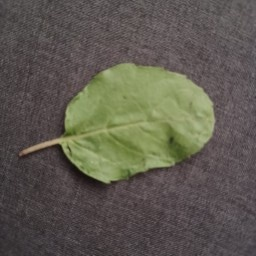
\includegraphics[width=0.2\columnwidth]{img/tulsi/tulsi1.jpg}%
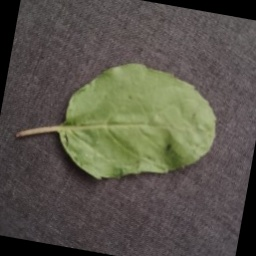
\includegraphics[width=0.2\columnwidth]{img/tulsi/tulsi2.jpg}%
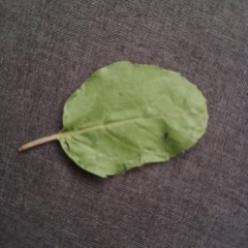
\includegraphics[width=0.2\columnwidth]{img/tulsi/tulsi3.jpg}%
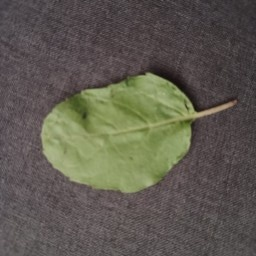
\includegraphics[width=0.2\columnwidth]{img/tulsi/tulsi4.jpg}%
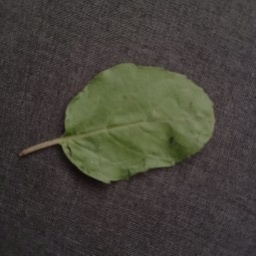
\includegraphics[width=0.2\columnwidth]{img/tulsi/tulsi5.jpg}\\[-0.5pt]
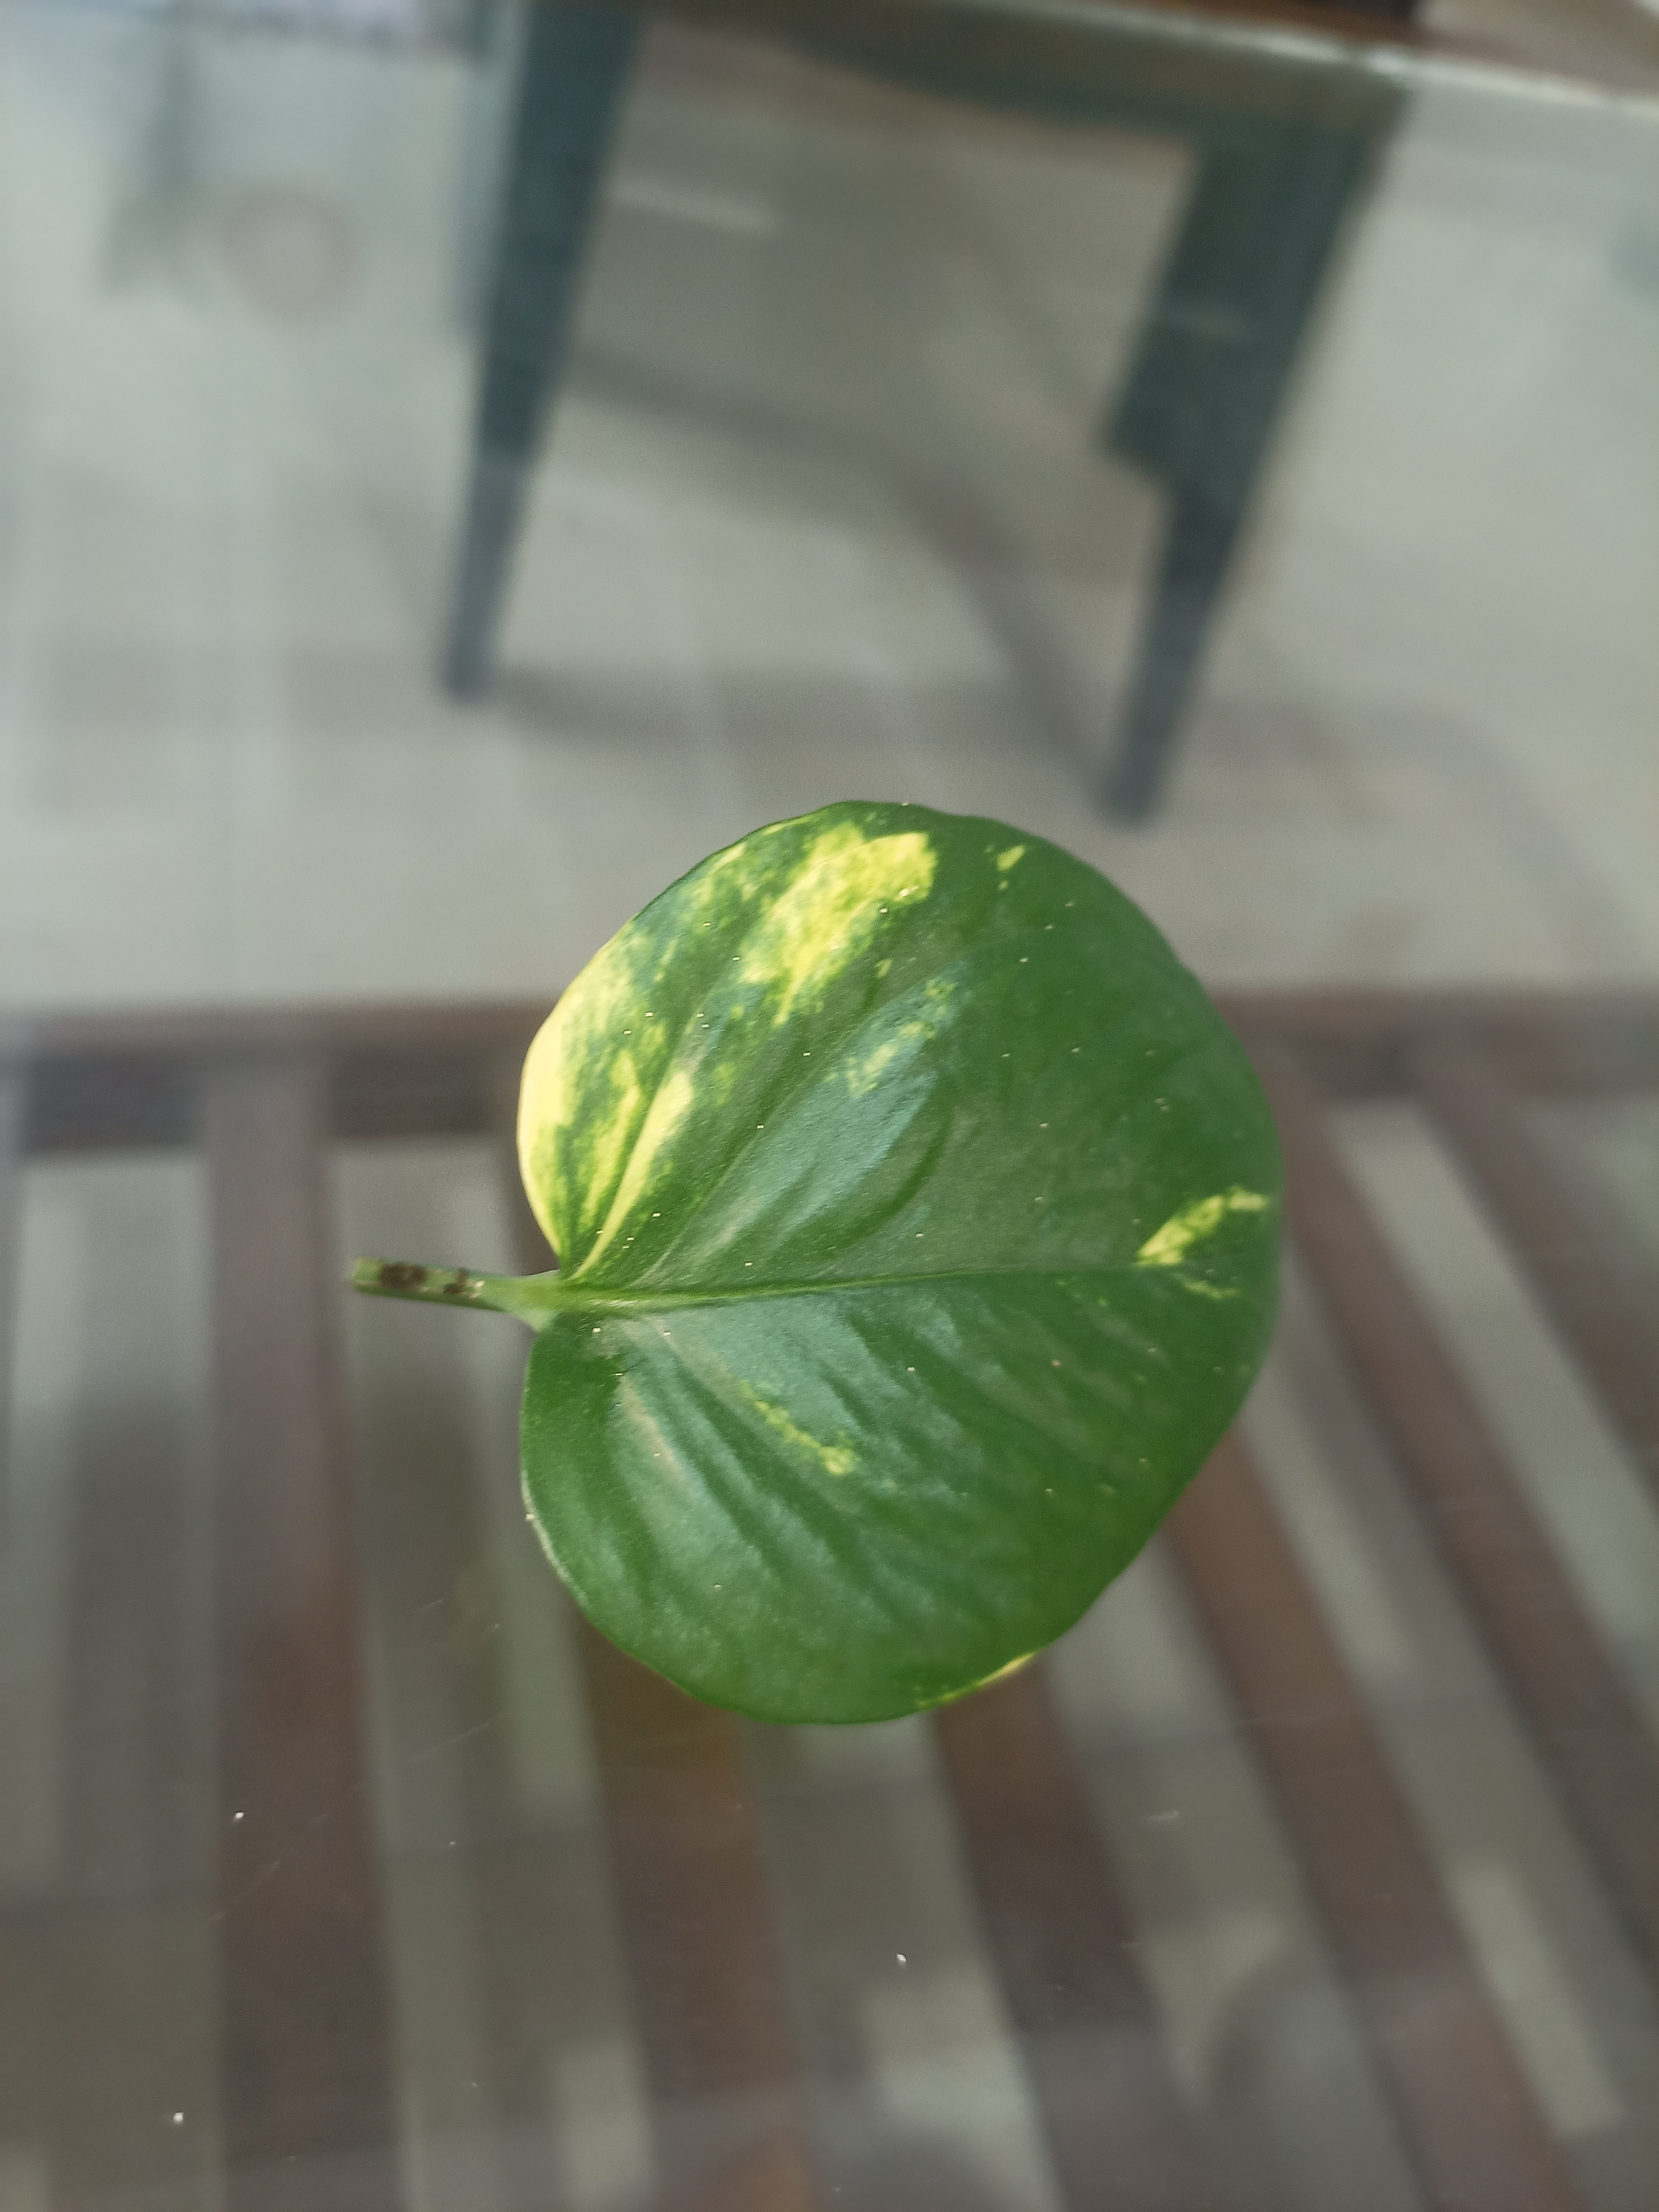
\includegraphics[width=0.2\columnwidth]{img/money/money1.jpg}%
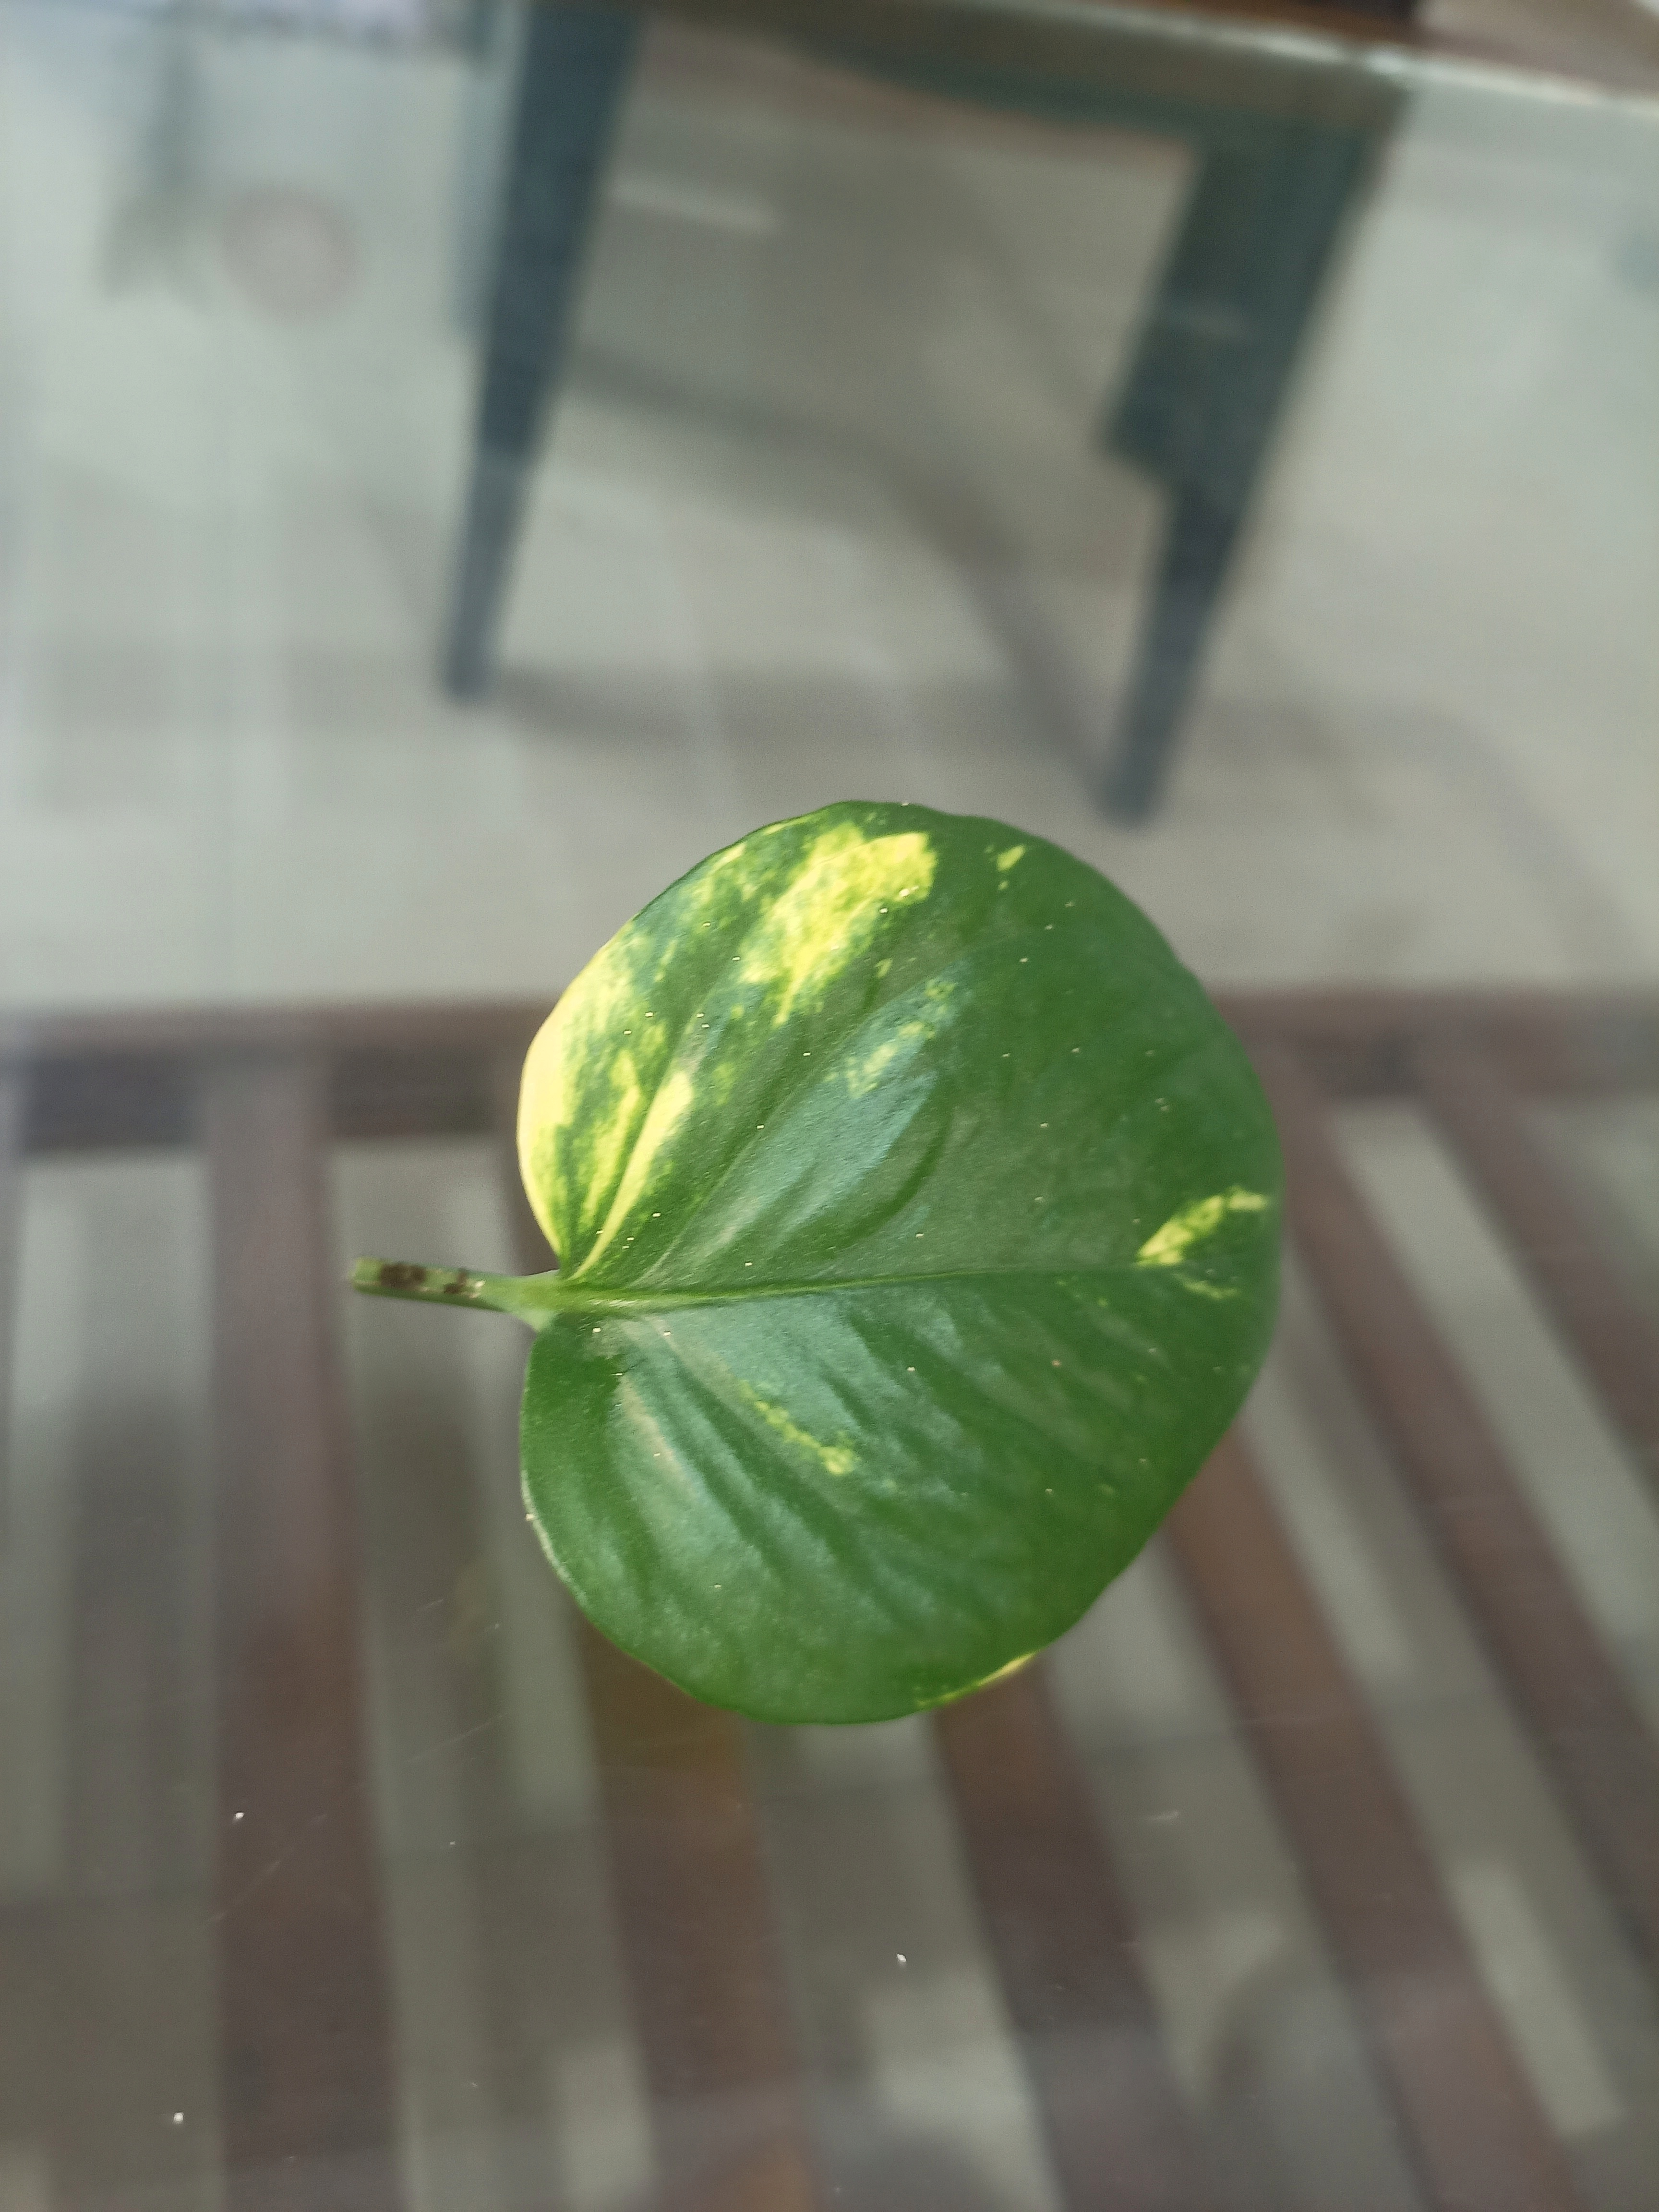
\includegraphics[width=0.2\columnwidth]{img/money/money2.jpg}%
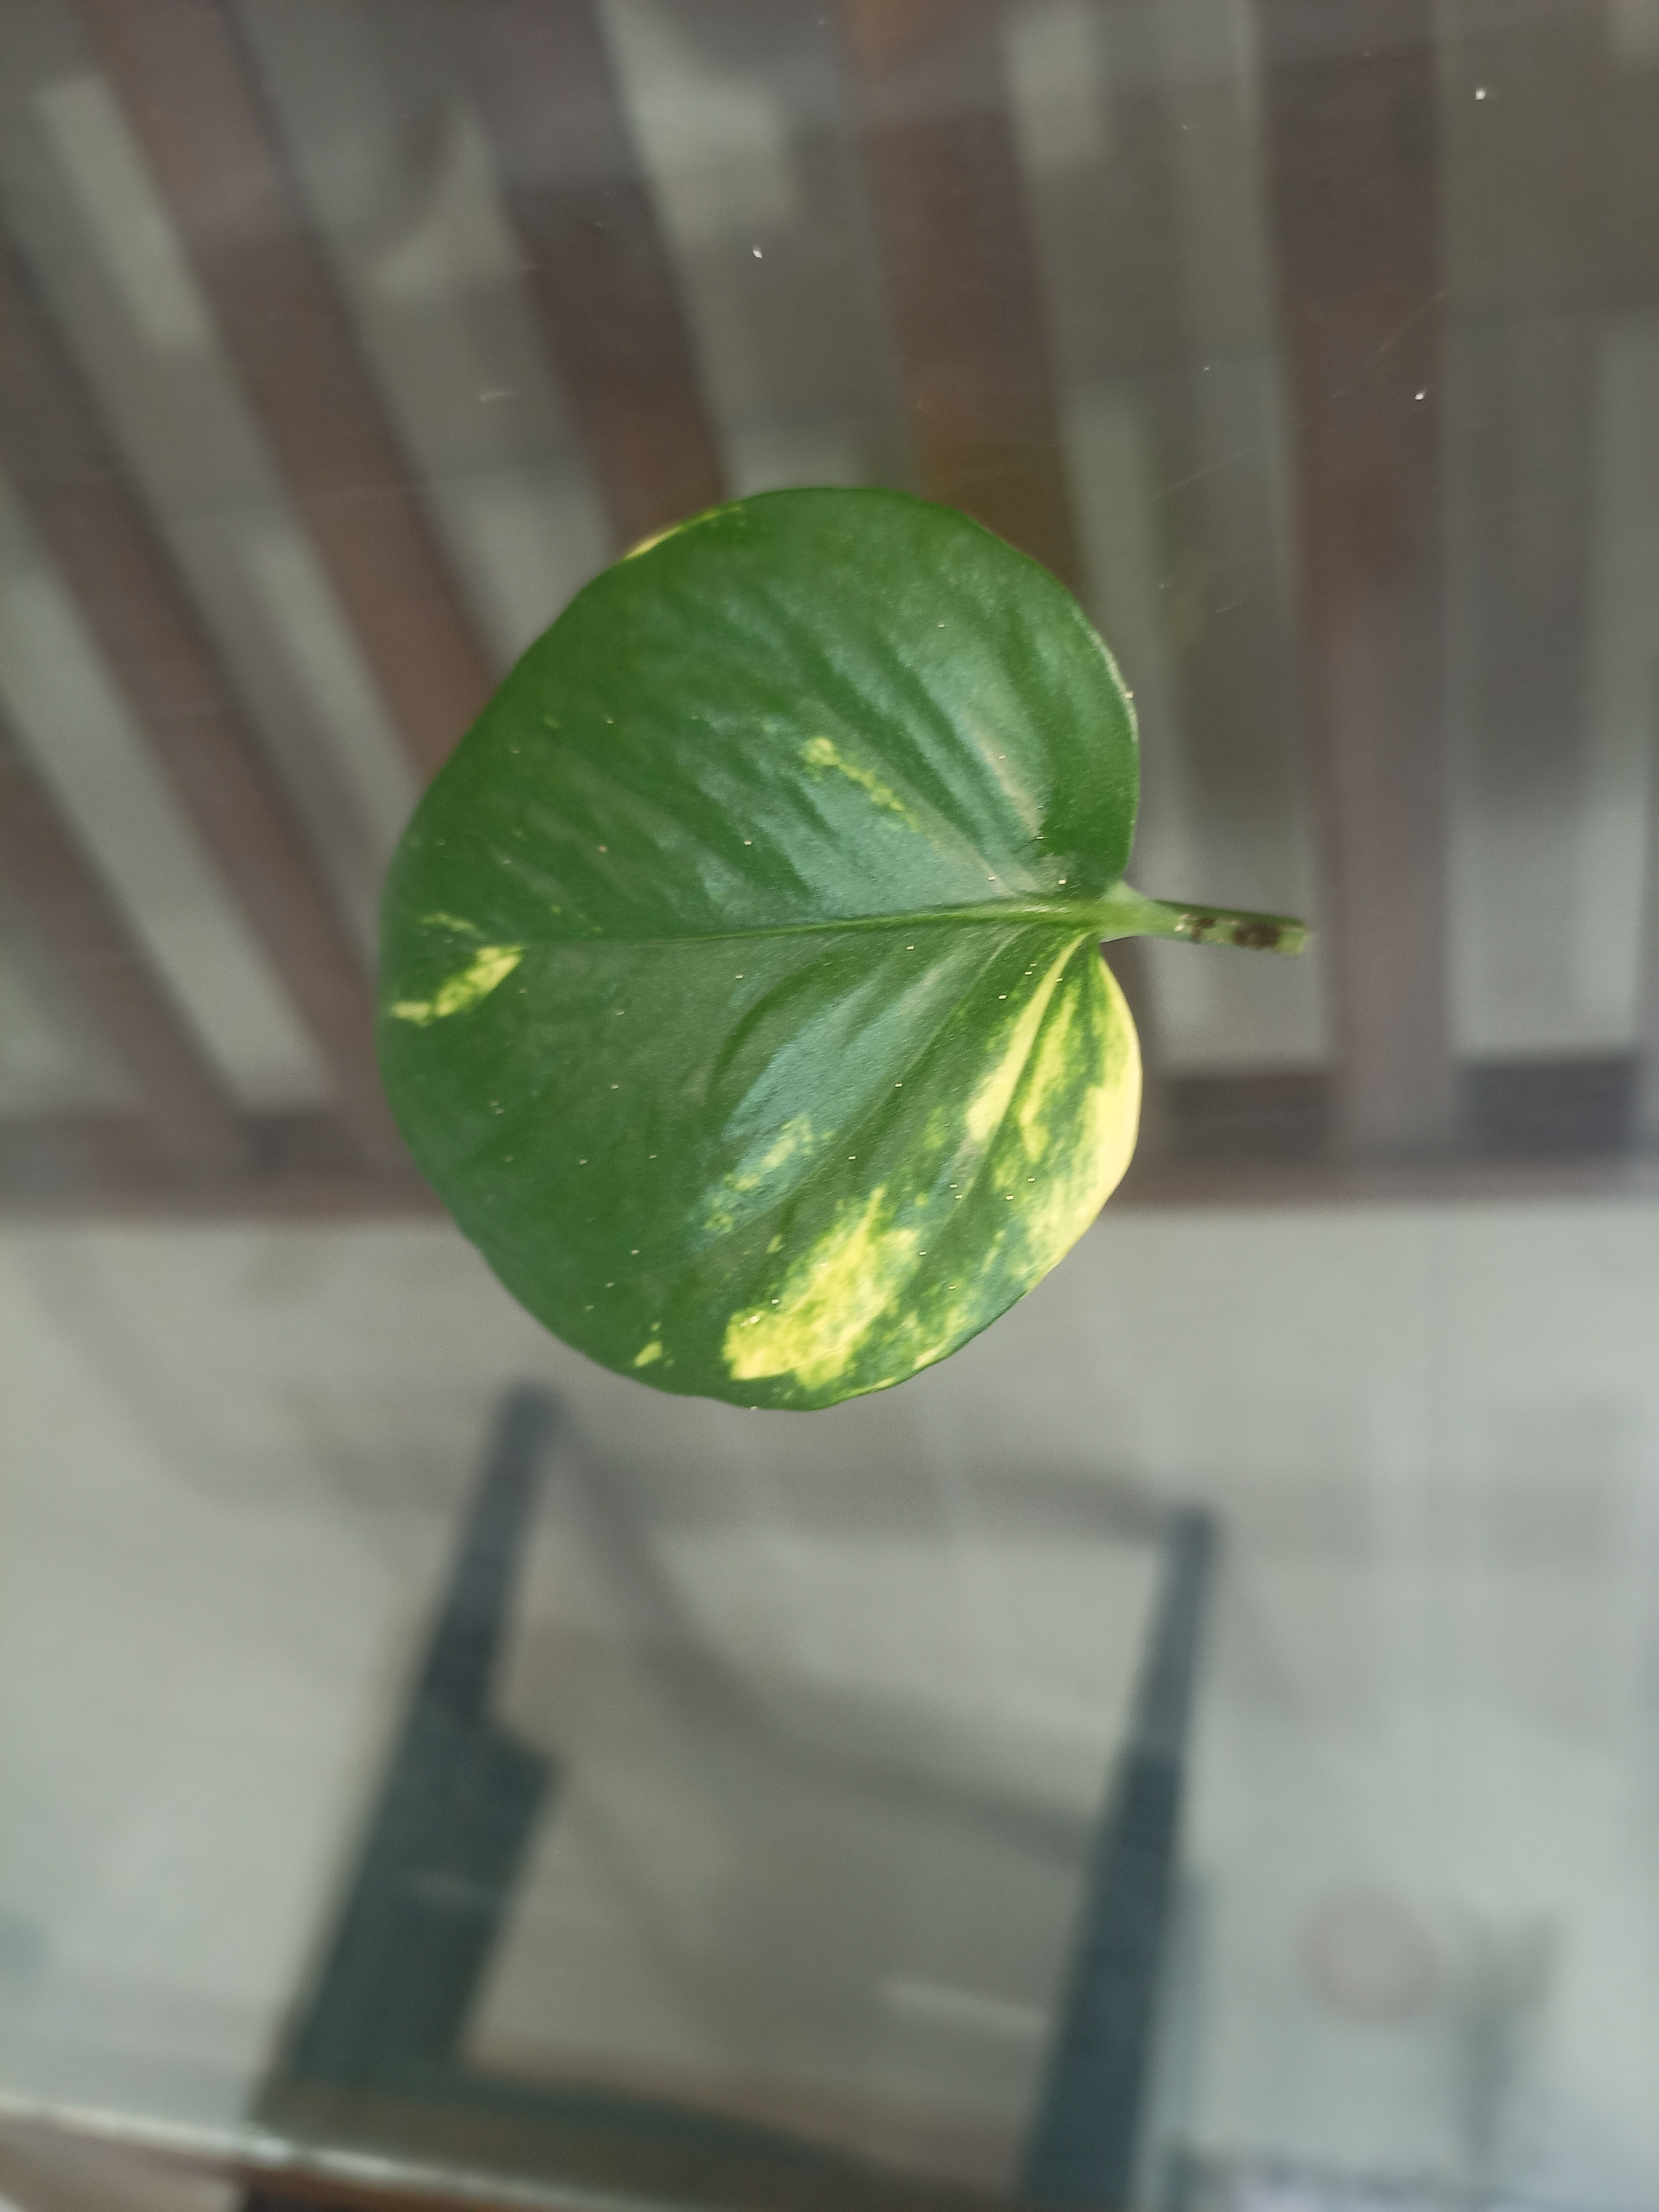
\includegraphics[width=0.2\columnwidth]{img/money/money3.jpg}%
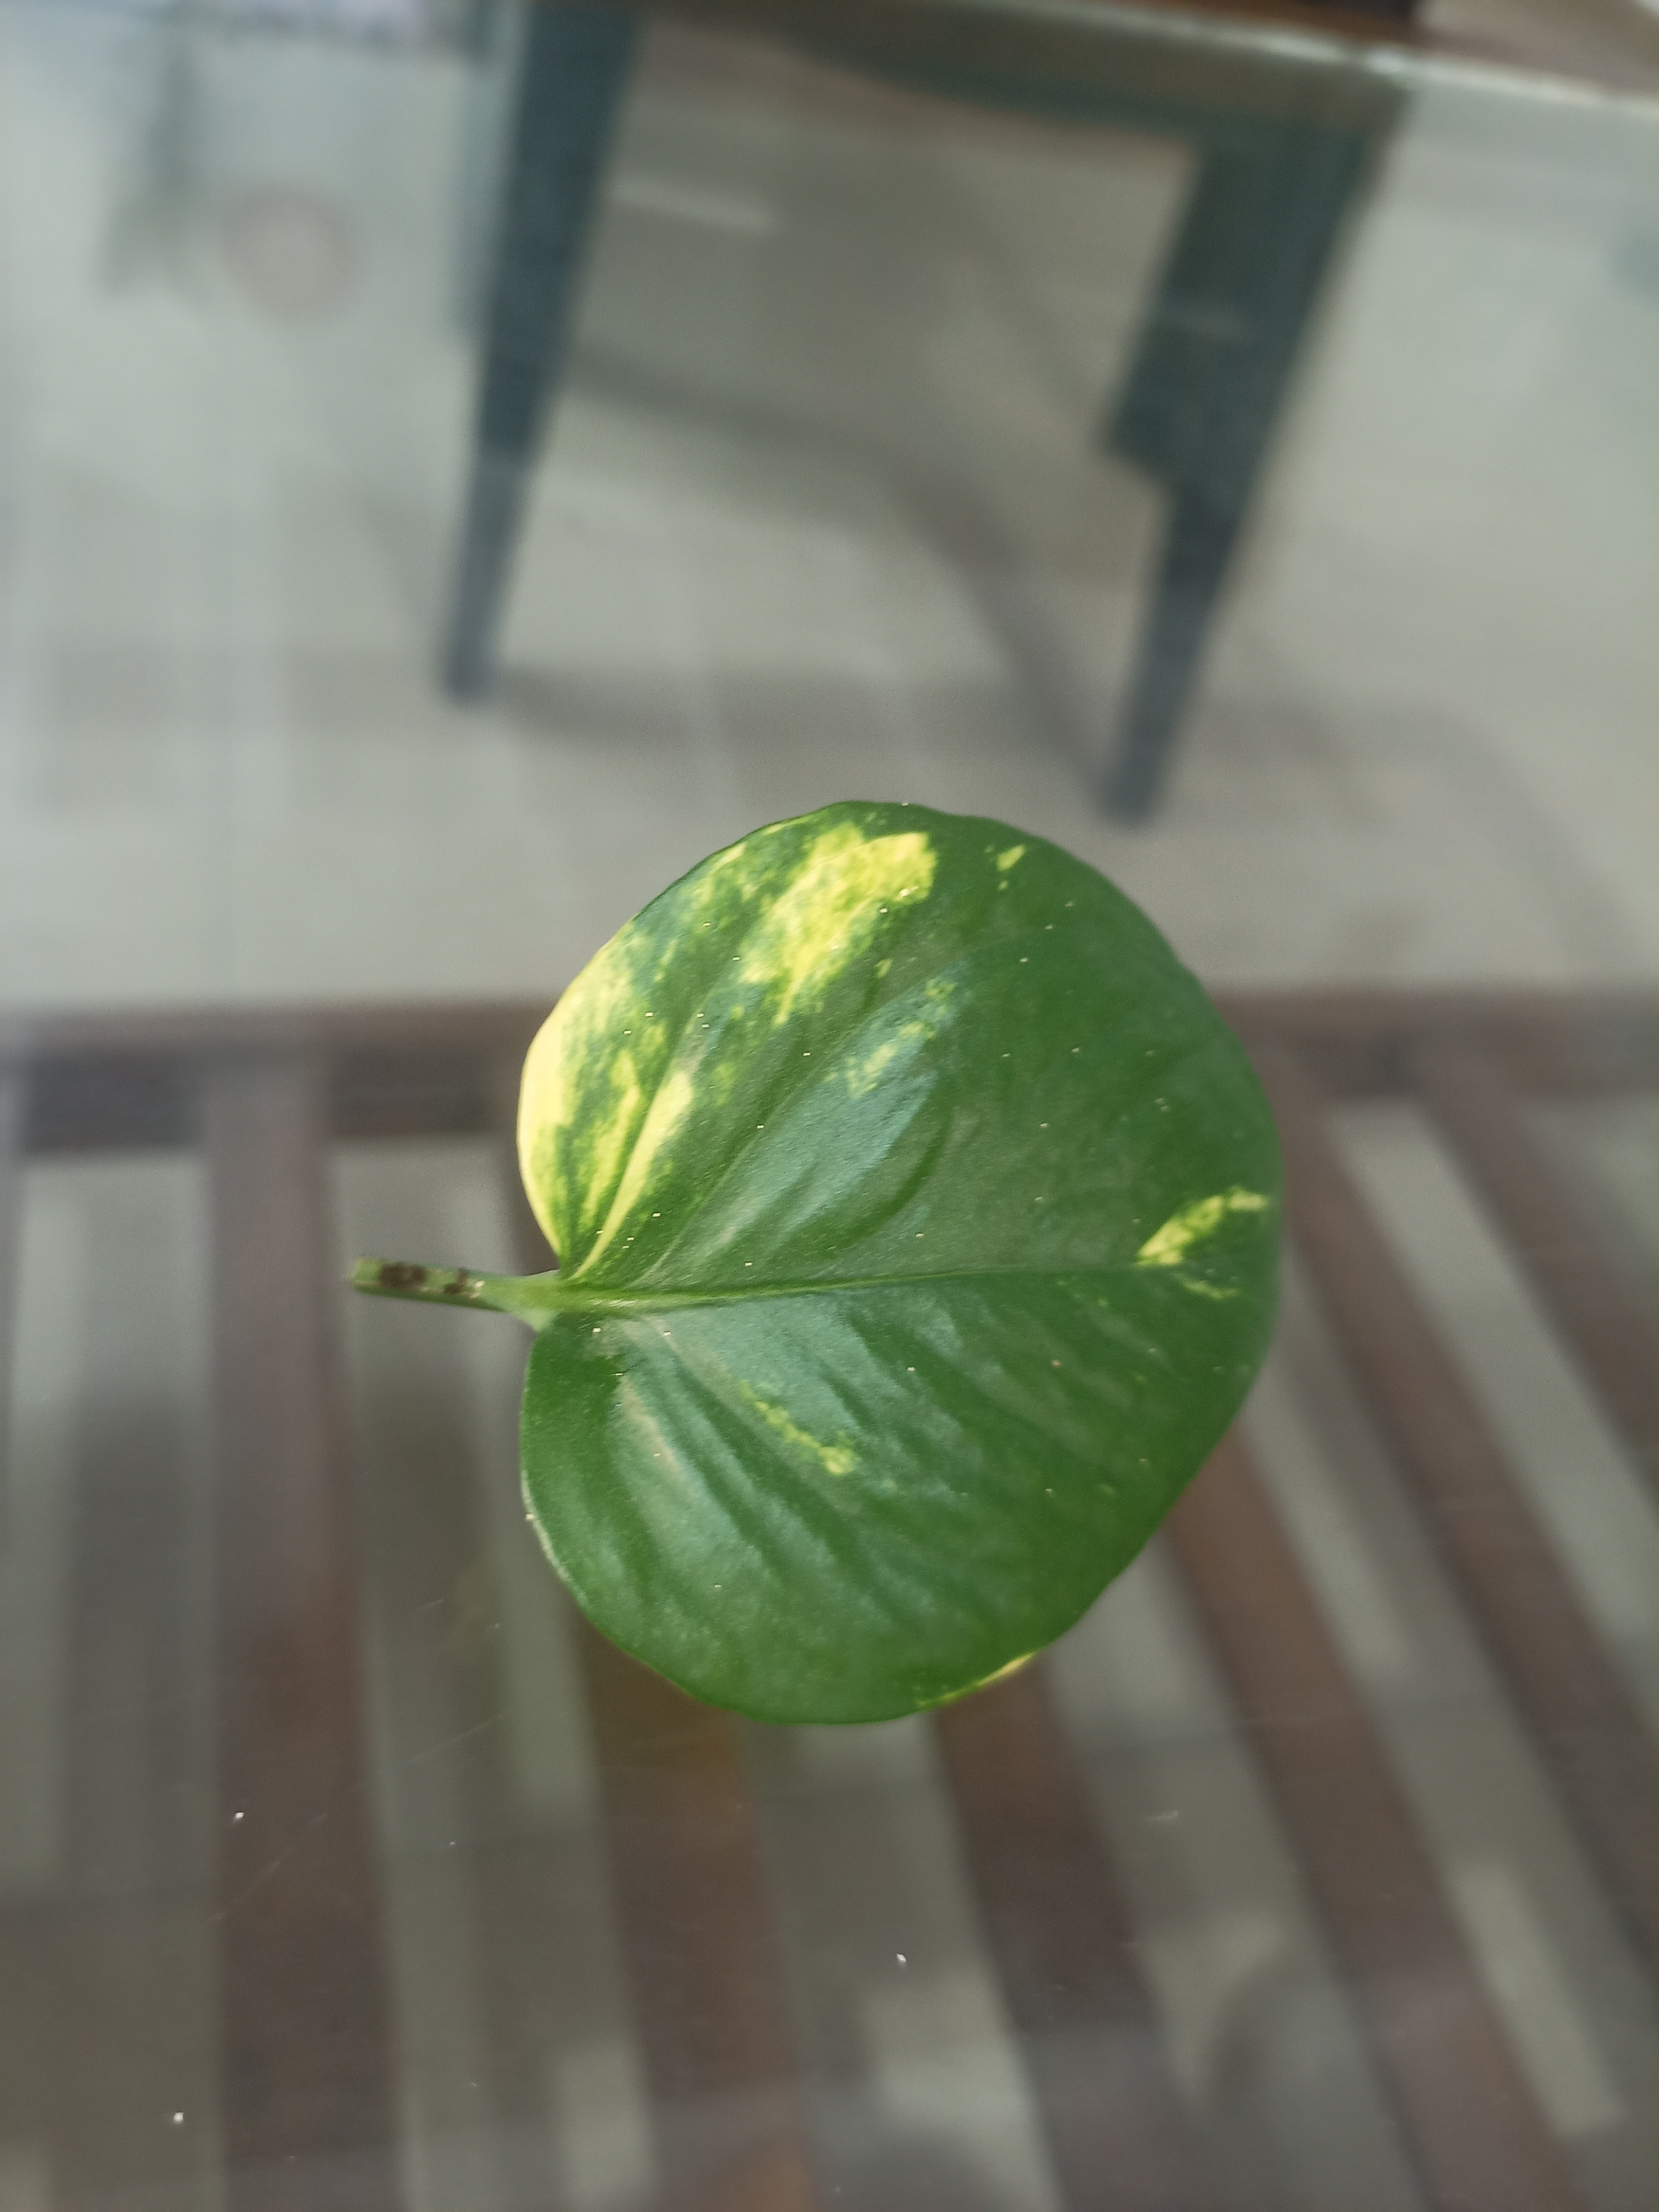
\includegraphics[width=0.2\columnwidth]{img/money/money4.jpg}%
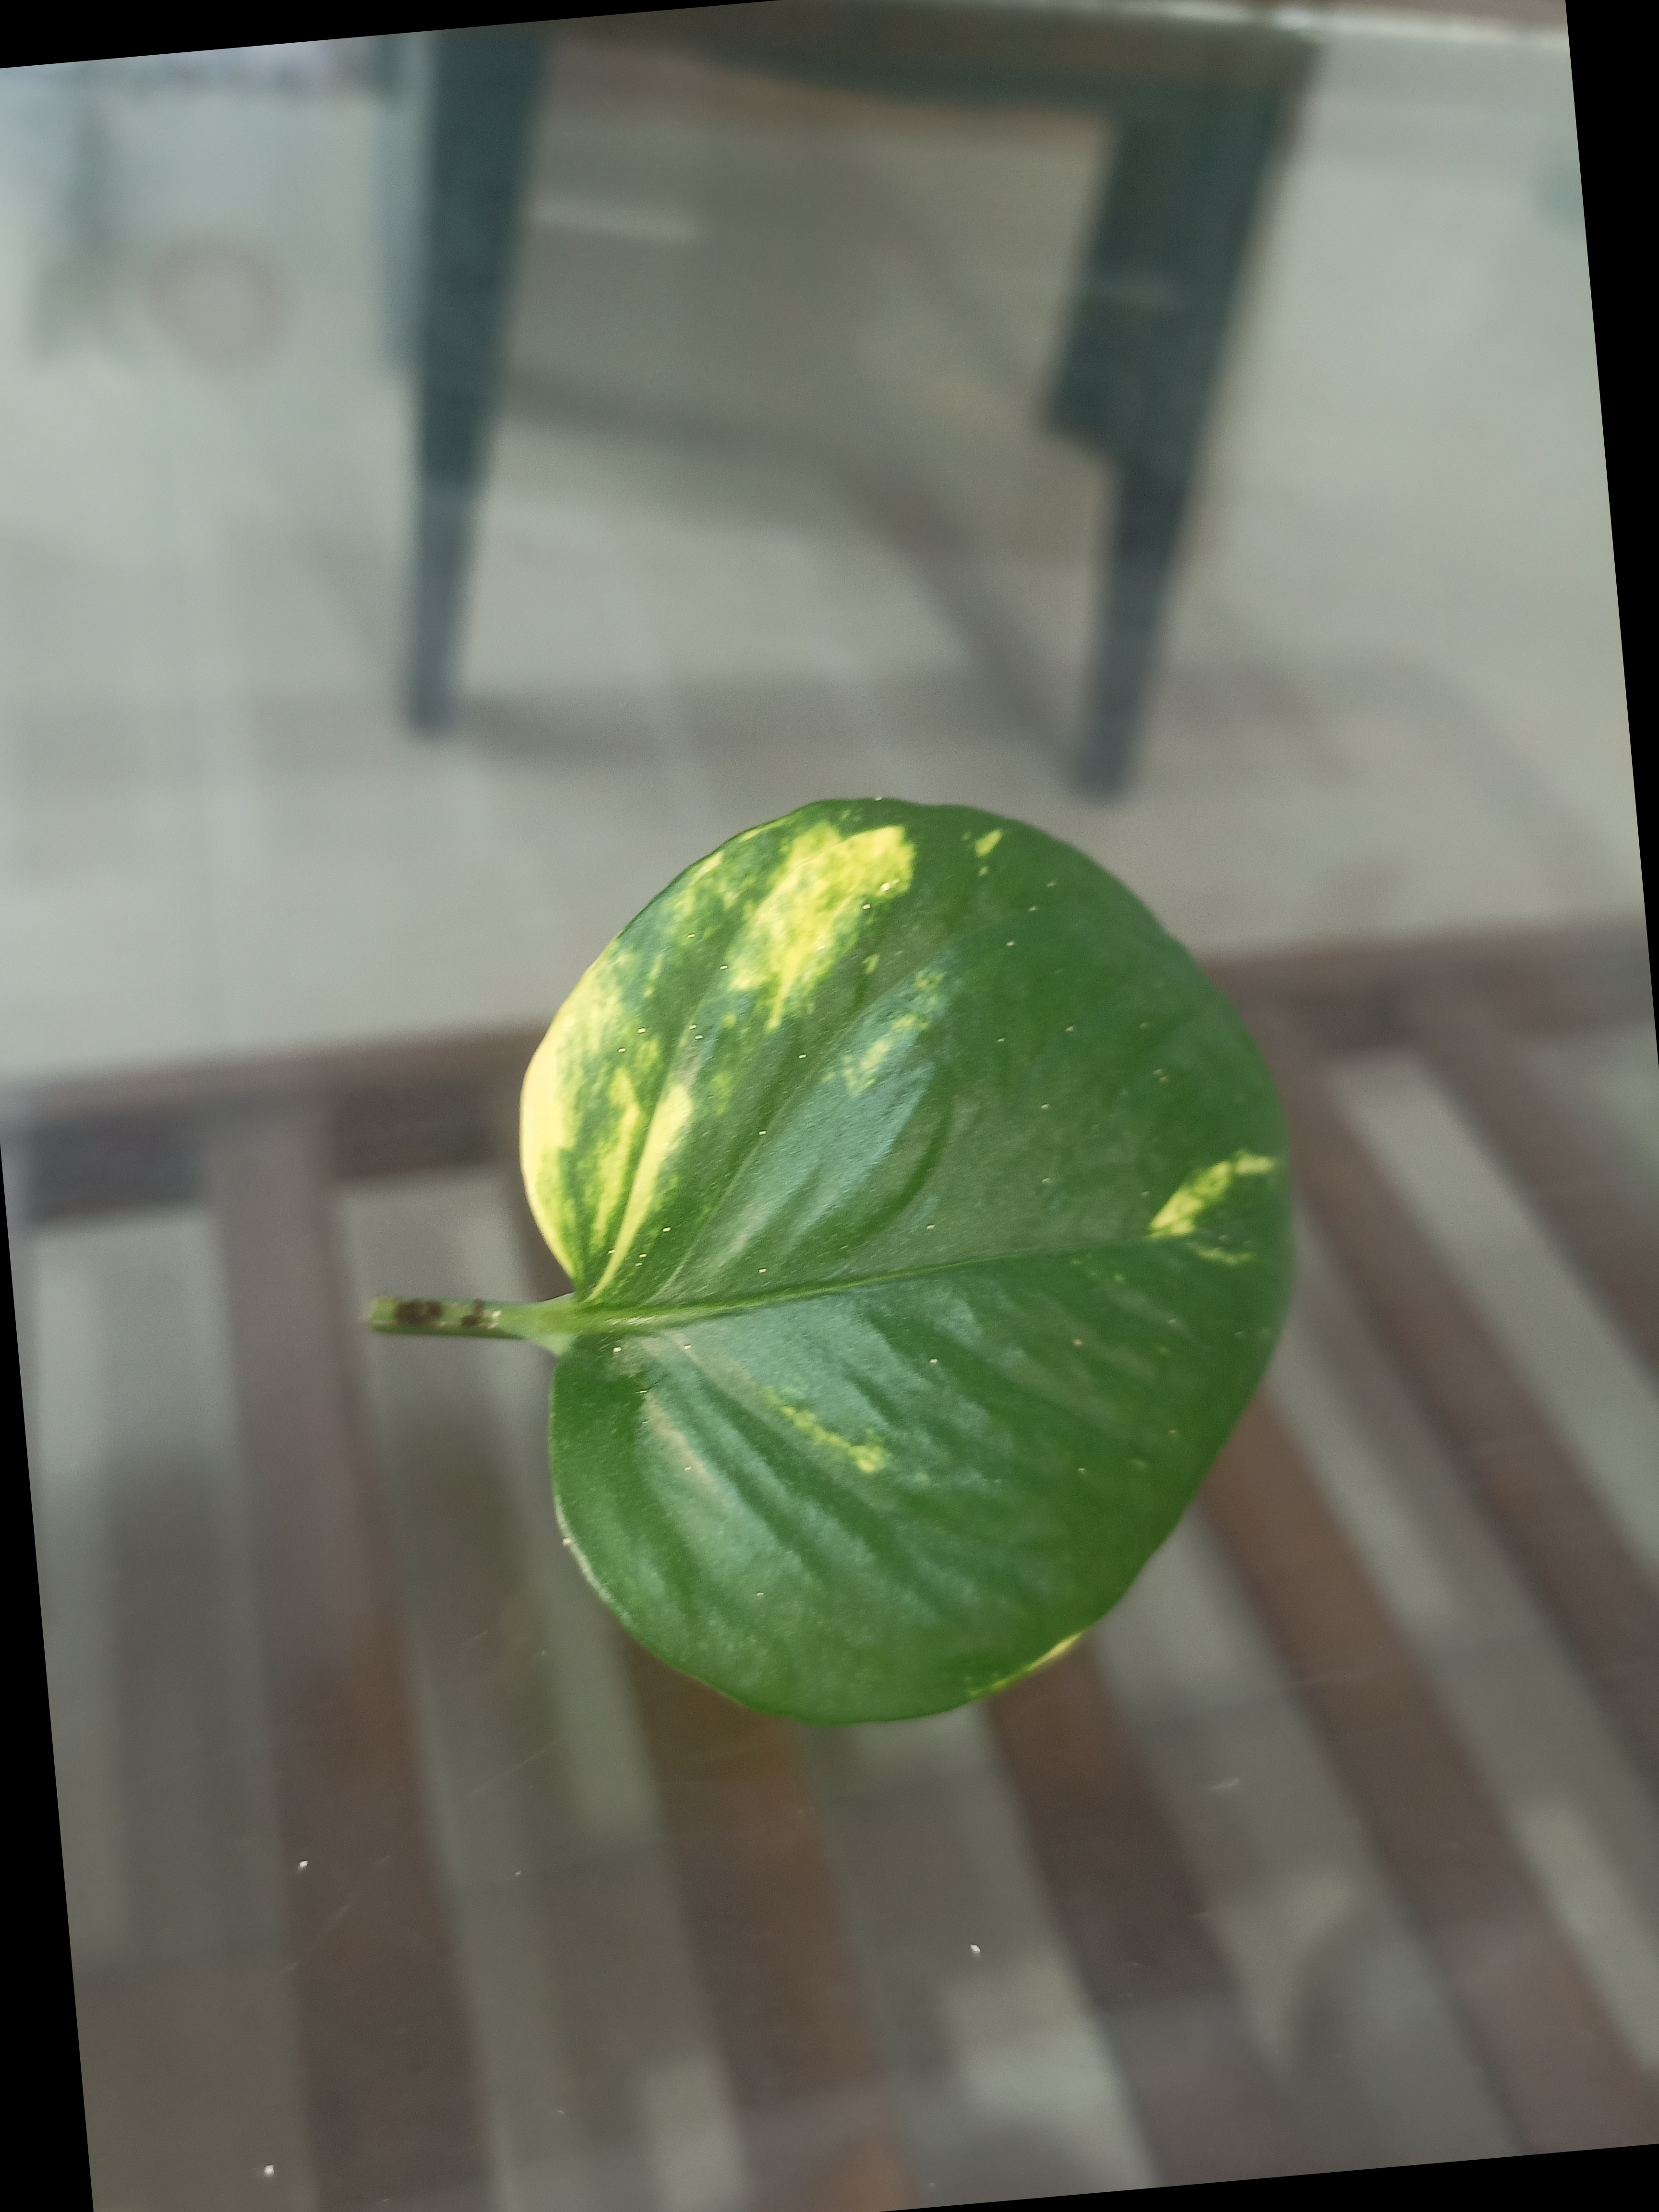
\includegraphics[width=0.2\columnwidth]{img/money/money5.jpg}\\[-0.5pt]
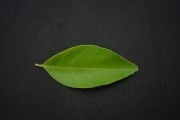
\includegraphics[width=0.2\columnwidth]{img/lemon/lemon1.jpg}%
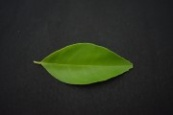
\includegraphics[width=0.2\columnwidth]{img/lemon/lemon2.jpg}%
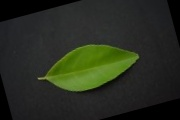
\includegraphics[width=0.2\columnwidth]{img/lemon/lemon3.jpg}%
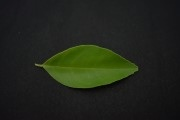
\includegraphics[width=0.2\columnwidth]{img/lemon/lemon4.jpg}%
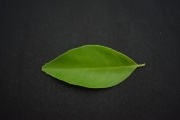
\includegraphics[width=0.2\columnwidth]{img/lemon/lemon5.jpg}\\[-0.5pt]
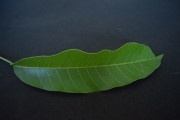
\includegraphics[width=0.2\columnwidth]{img/mango/mango1.jpg}%
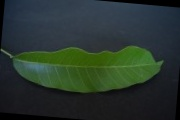
\includegraphics[width=0.2\columnwidth]{img/mango/mango2.jpg}%
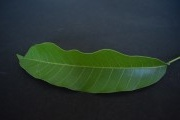
\includegraphics[width=0.2\columnwidth]{img/mango/mango3.jpg}%
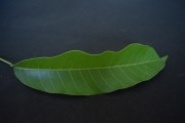
\includegraphics[width=0.2\columnwidth]{img/mango/mango4.jpg}%
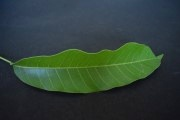
\includegraphics[width=0.2\columnwidth]{img/mango/mango5.jpg}\\[-0.5pt]
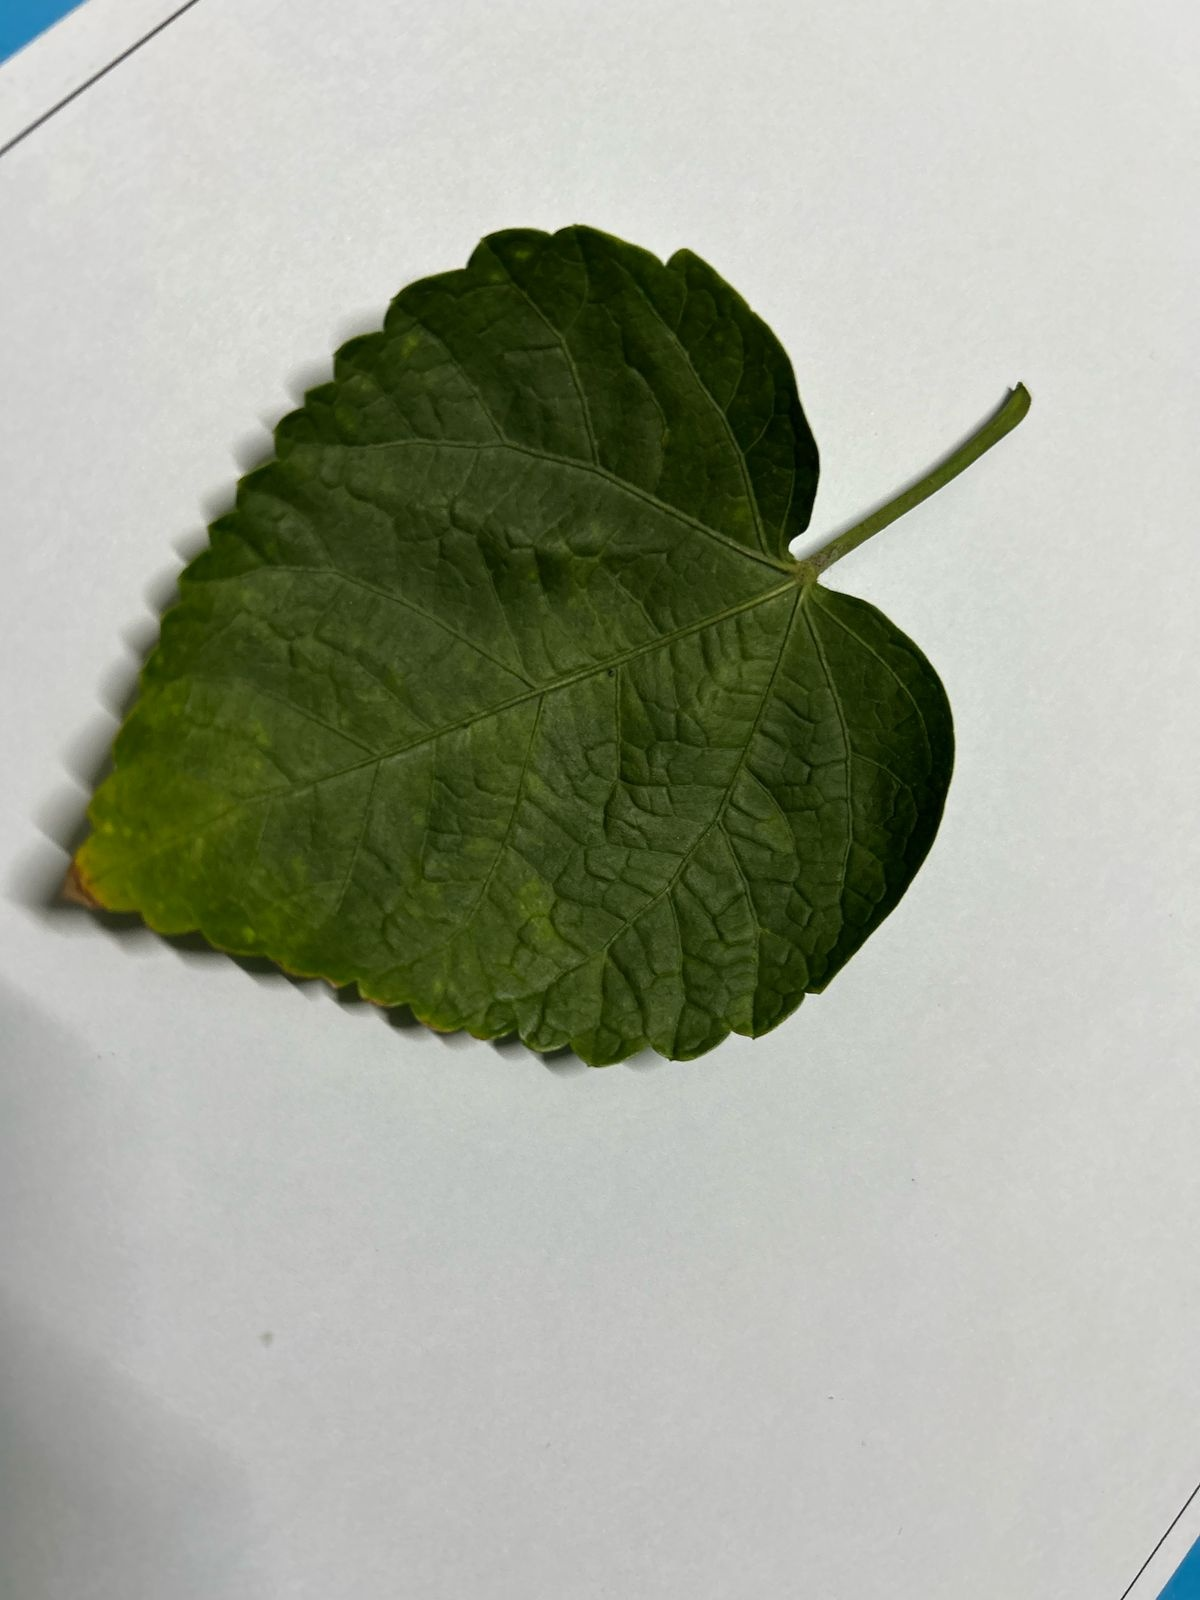
\includegraphics[width=0.2\columnwidth]{img/rosa/rosa1.jpg}%
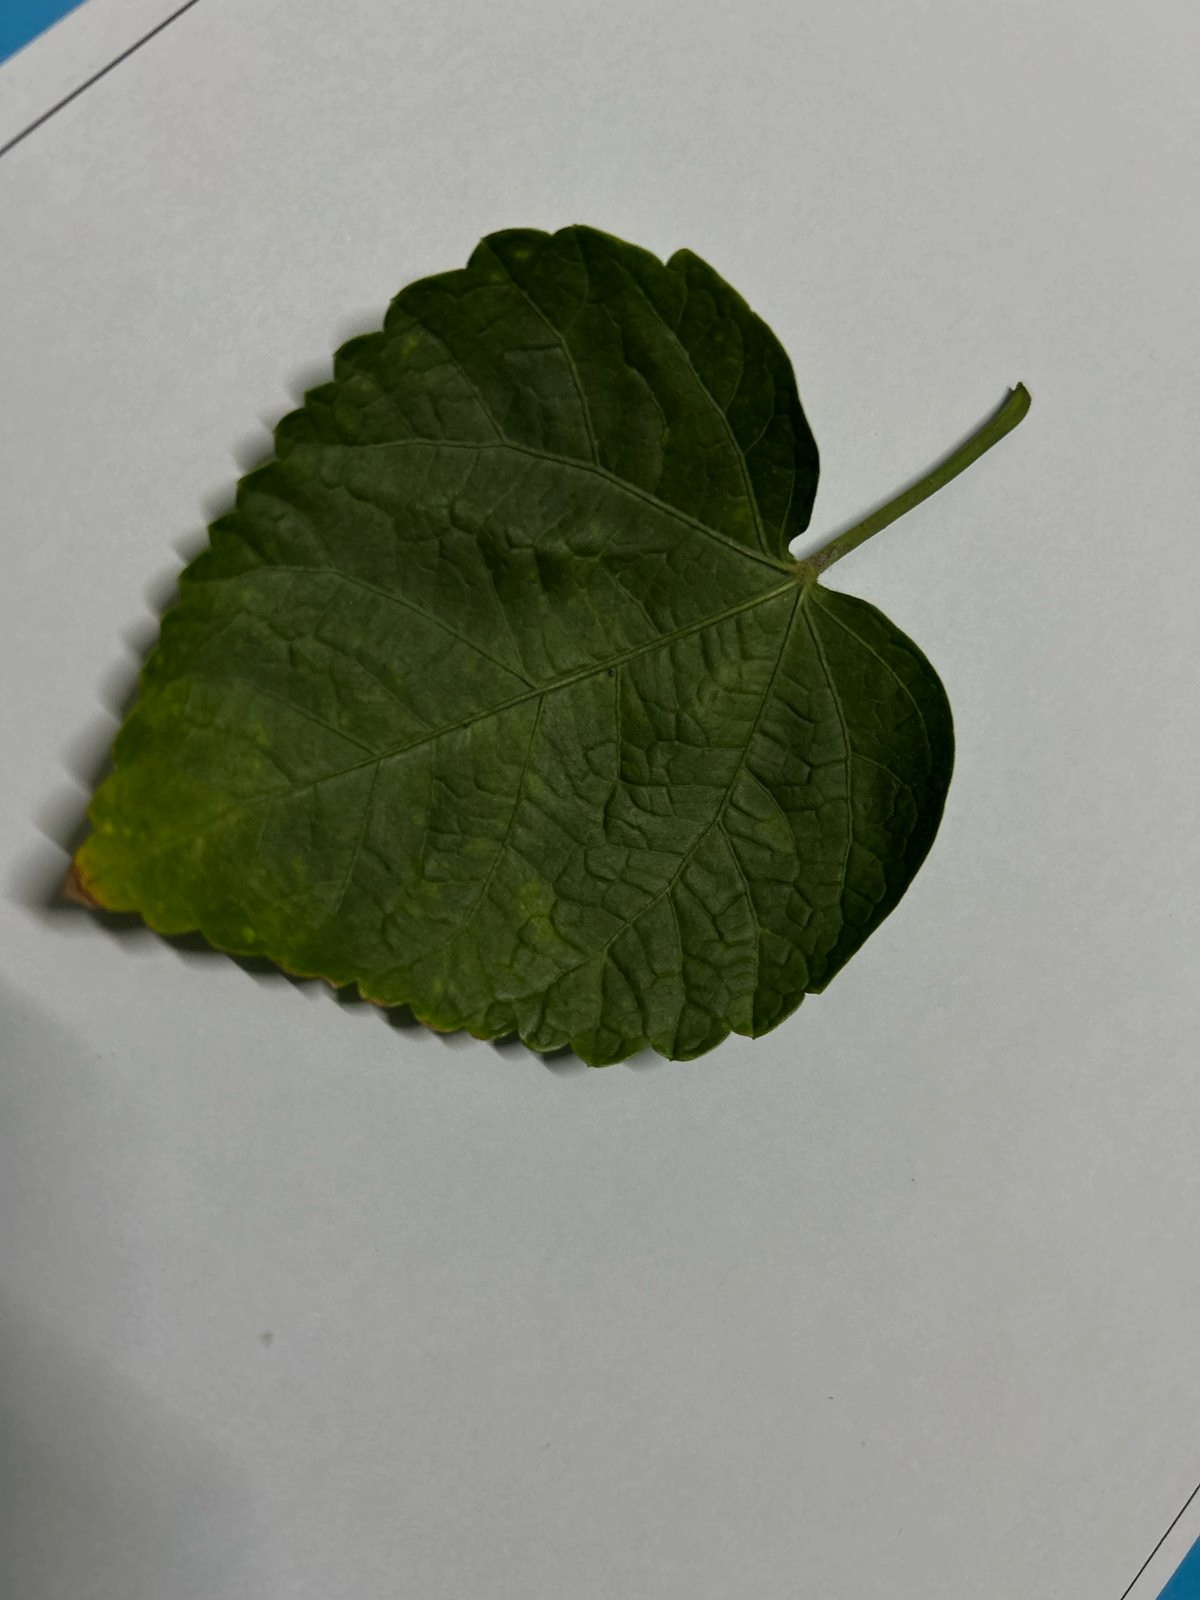
\includegraphics[width=0.2\columnwidth]{img/rosa/rosa2.jpg}%
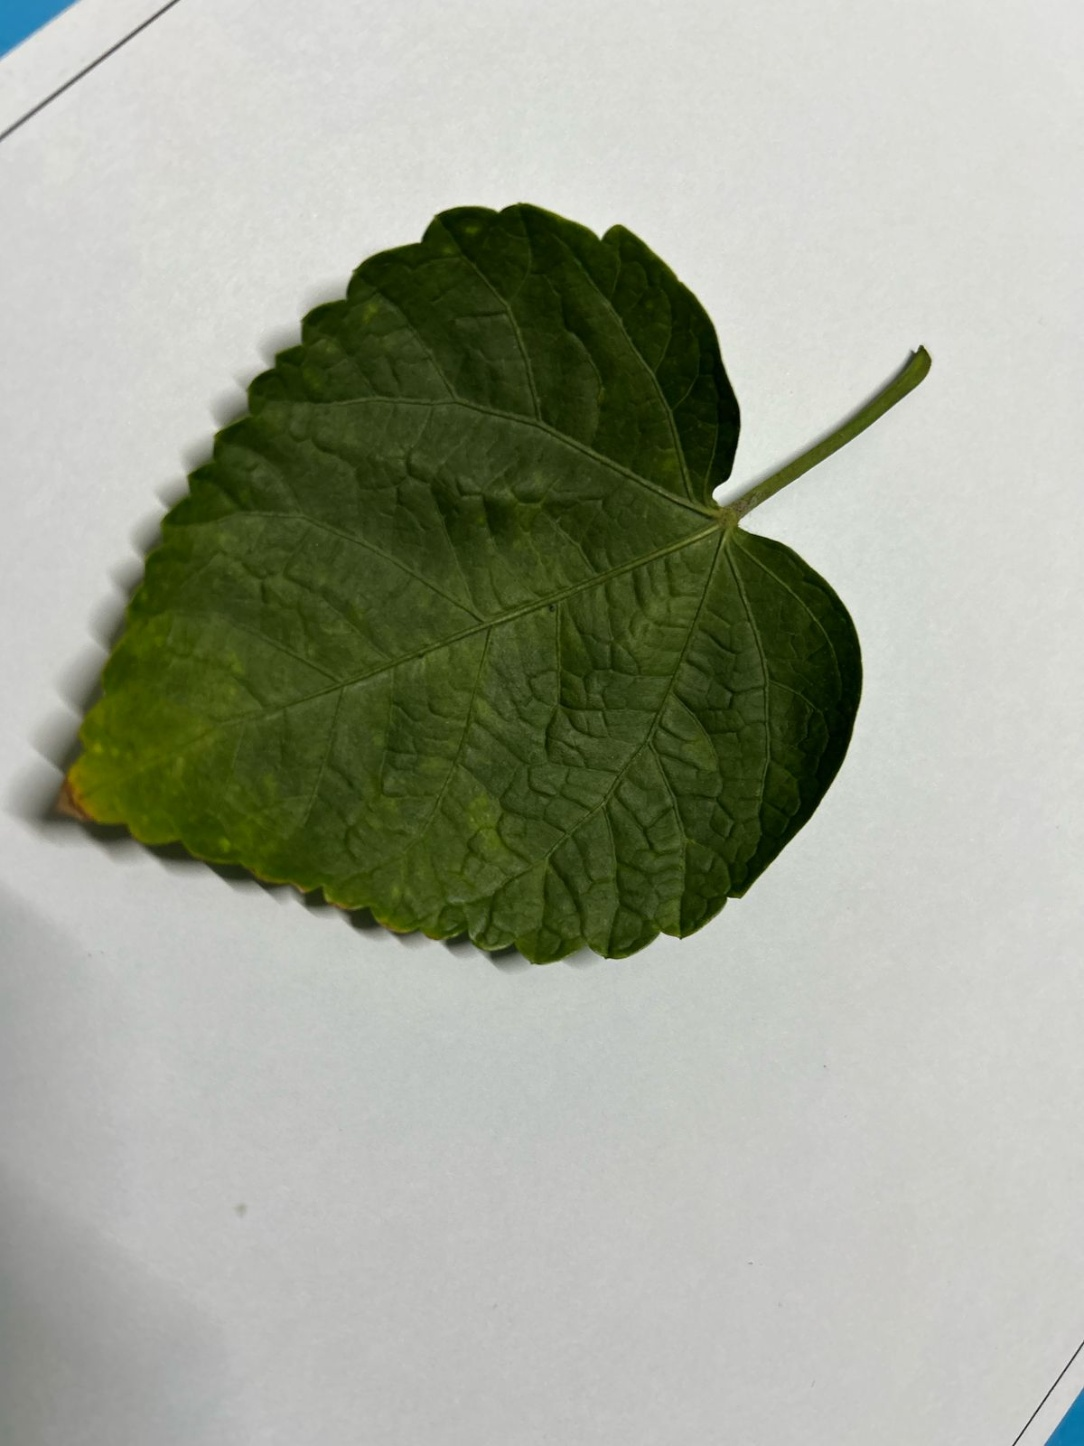
\includegraphics[width=0.2\columnwidth]{img/rosa/rosa3.jpg}%
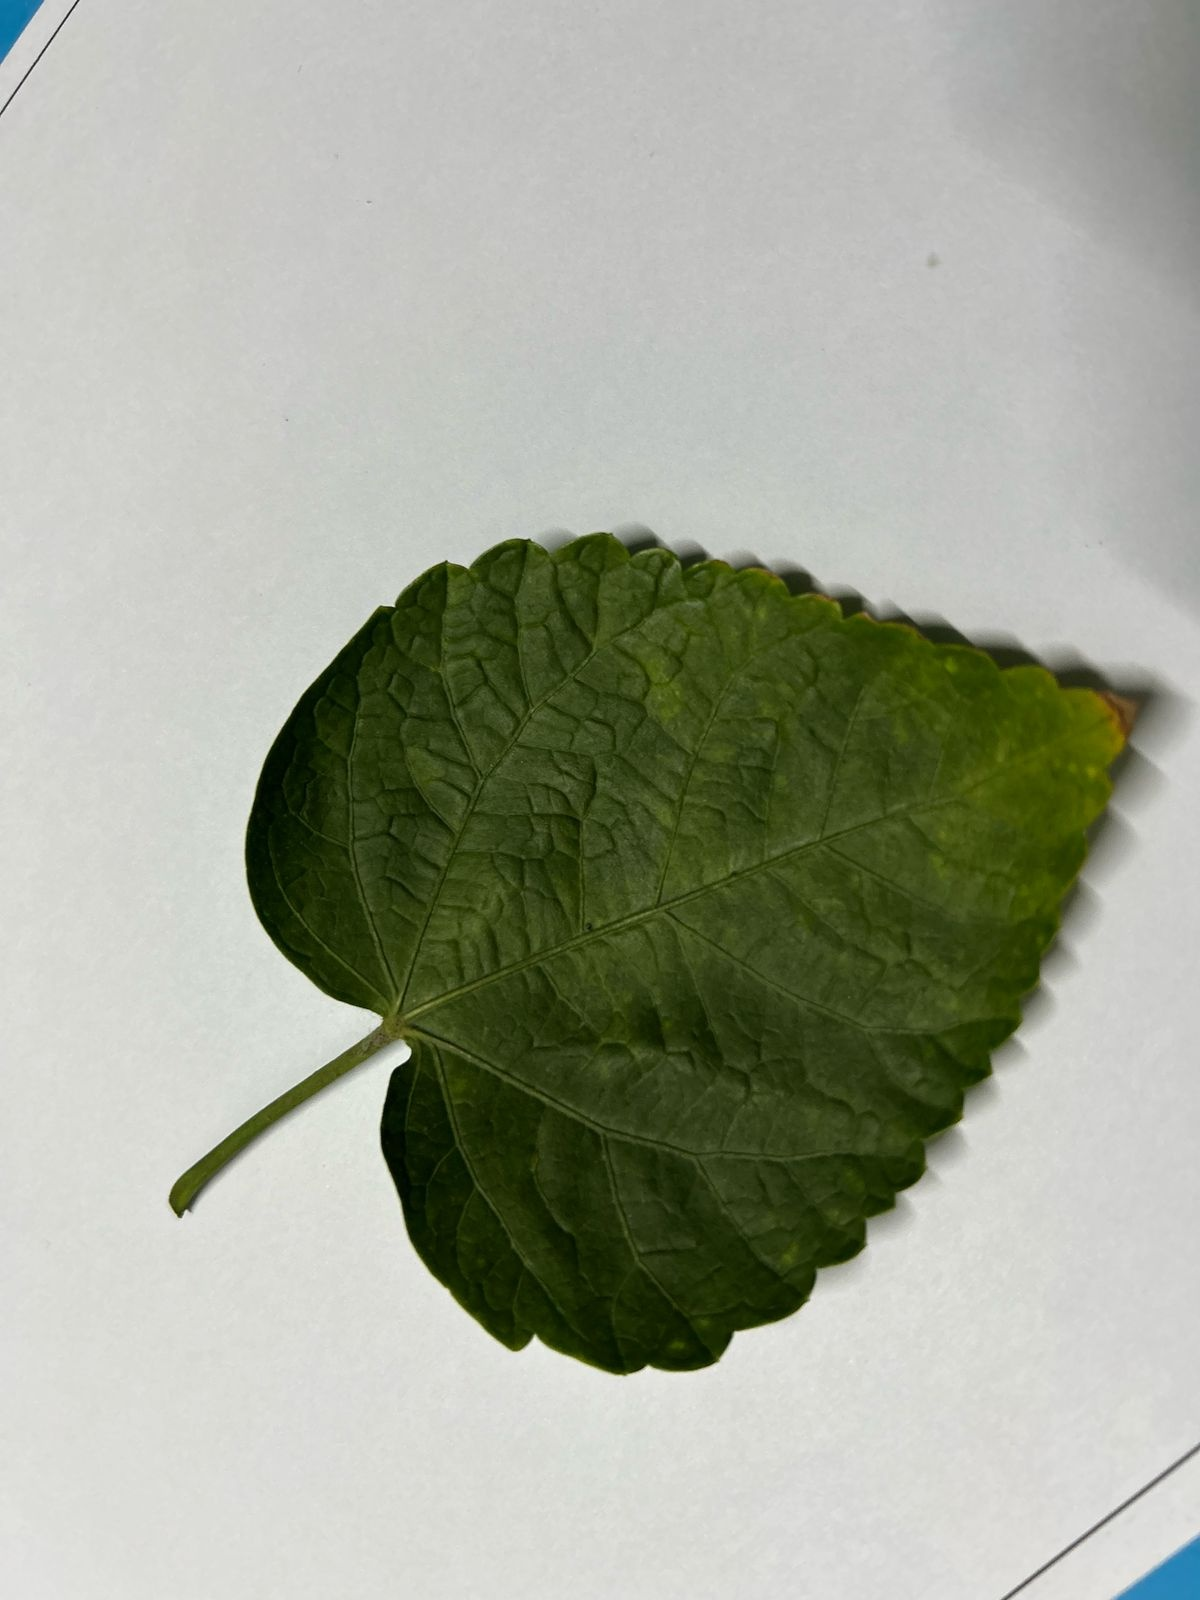
\includegraphics[width=0.2\columnwidth]{img/rosa/rosa4.jpg}%
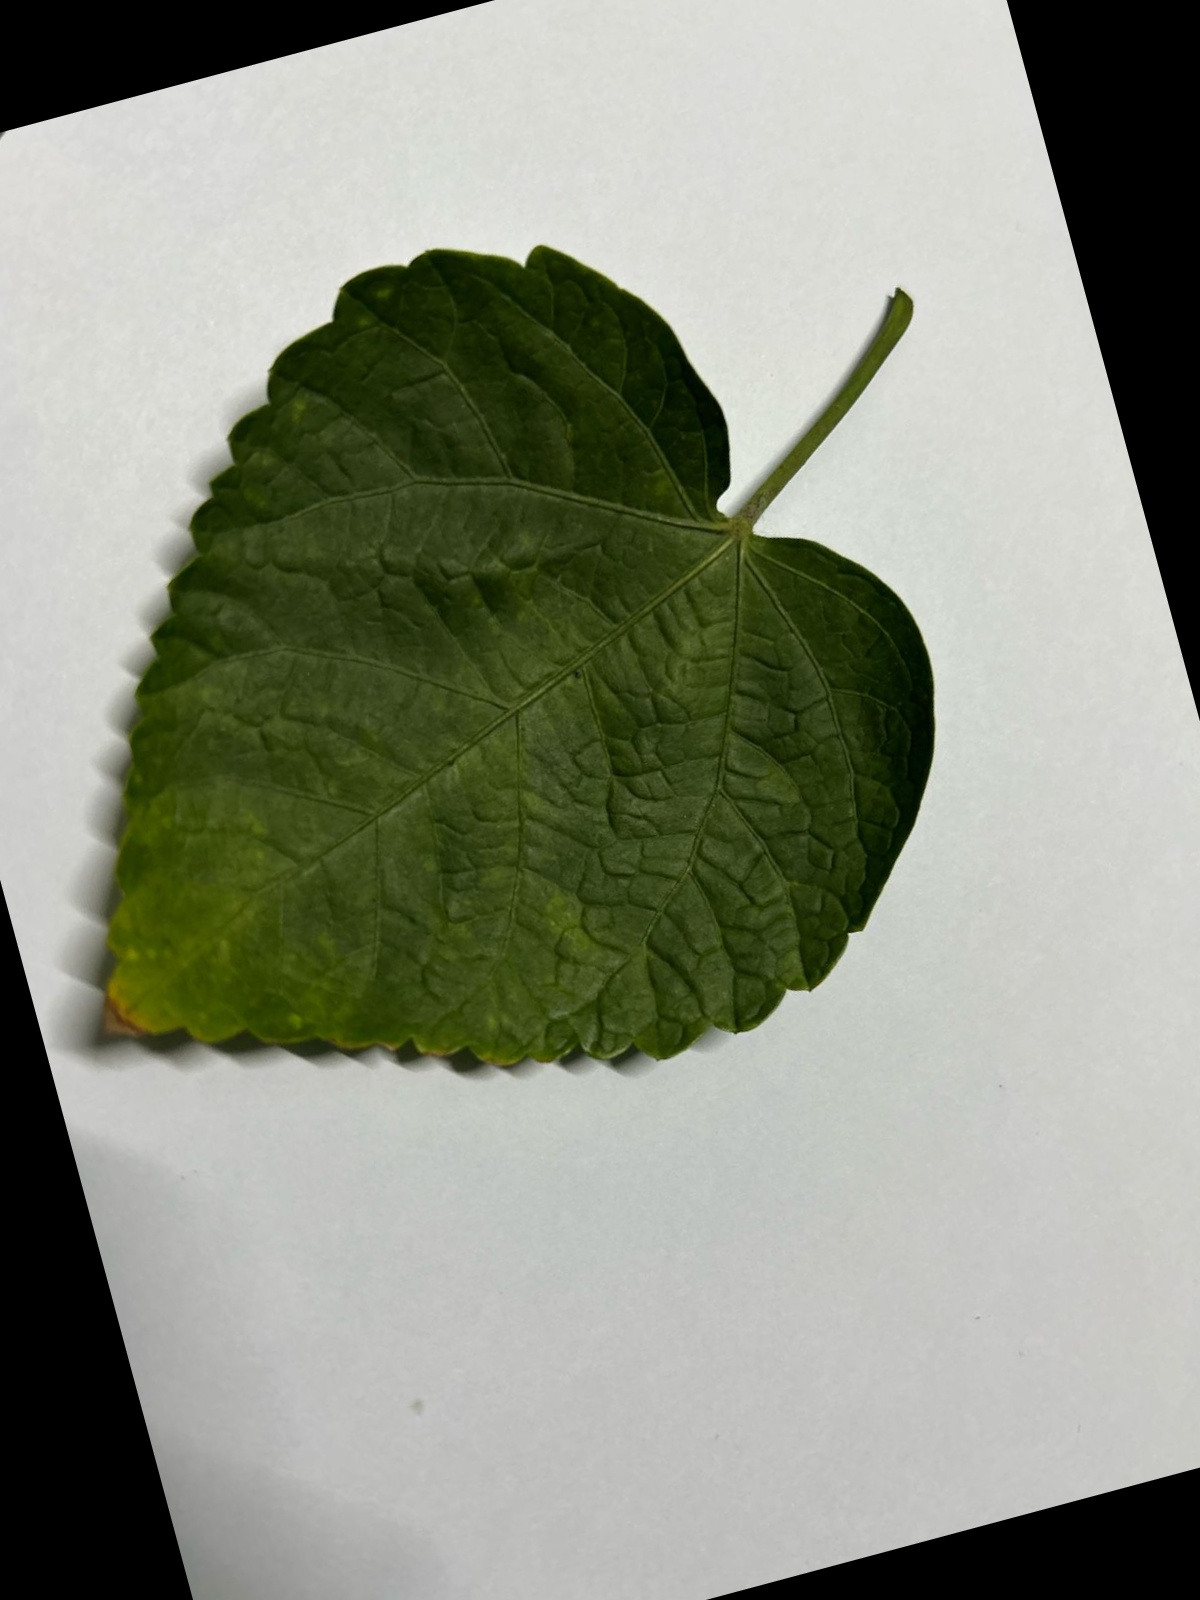
\includegraphics[width=0.2\columnwidth]{img/rosa/rosa5.jpg}
\end{minipage}
\caption{Images of five different plant leaves (tulsi, money plant, lemon, mango, rosa-senensis).}
\label{fig:sample-images}
\end{figure}



\section{Model Training}
To train the model, we built a Convolutional Neural Network (CNN) using TensorFlow and Keras. The architecture consisted of three convolutional layers with ReLU activation, followed by max pooling layers. After flattening, we added a dense layer with 64 neurons and a dropout layer to prevent overfitting. The final output layer had three neurons with a softmax activation function to classify the images into three categories. The model was compiled using the Adam optimizer and categorical cross-entropy loss, and it was trained for 50 epochs.

\section{Detailed CNN Architecture}
Our CNN models process 252x252 sized input images with three color channels (RGB). The architecture consists of:

\begin{itemize}\itemsep4pt
    \item \textbf{Input Layer}: Accepts 252x252 RGB images without any learning parameters.
    
    \item \textbf{First Convolutional Block}:
    \begin{itemize}\itemsep2pt
        \item Conv2D layer with 16 filters (3×3), ReLU activation
        \item Output size: (252, 252, 16)
        \item Parameters: 896
        \item MaxPooling2D (2×2) reduces dimensions to (126, 126, 16)
    \end{itemize}
    
    \item \textbf{Second Convolutional Block}:
    \begin{itemize}\itemsep2pt
        \item Conv2D layer with 32 filters (3×3), ReLU activation
        \item Output size: (61, 61, 32)
        \item Parameters: 18,496
        \item MaxPooling2D (2×2) reduces dimensions to (30, 30, 32)
    \end{itemize}
    
    \item \textbf{Third Convolutional Block}:
    \begin{itemize}\itemsep2pt
        \item Conv2D layer with 64 filters (3×3), ReLU activation
        \item Output size: (28, 28, 128)
        \item Parameters: 73,856
        \item MaxPooling2D (2×2) reduces dimensions to (14, 14, 128)
    \end{itemize}
    
    \item \textbf{Fully Connected Layers}:
    \begin{itemize}\itemsep2pt
        \item Flatten layer converts to 25,088 1D vectors
        \item Dense layer with 256 neurons, ReLU activation
        \item Parameters: 6,422,784
        \item Dropout layer (0.3)
        \item Output layer with 3 neurons, softmax activation
        \item Parameters: 1,285
    \end{itemize}
\end{itemize}

Total Parameters: 13,872,707

\section{Testing and Evaluation}
We tested our model over 100 epochs to measure its performance. The model reached 97\% accuracy on training data but only 85-89\% on validation data. This gap shows overfitting happened even with dropout regularization in place. The validation accuracy changed a lot during training, showing uneven performance on new data. Training loss went down steadily to below 0.1, while validation loss stayed around 0.5 with many ups and downs.

These results show that the model works well with leaf images it has seen before but has trouble with new examples. To fix this problem, we will try more regularization techniques or better data augmentation methods. These changes would help build a more reliable leaf classification system that works well with all types of images.

\section{Results}
\subsection{Model Performance}
Key metrics:
\begin{itemize}\itemsep4pt
    \item CNN Model Accuracy: 91.1\% (Test Set)
    \item Loss: 0.21 (Cross-Entropy)
    \item Training accuracy improved significantly after 50 epochs
    \item Loss decreased steadily, indicating a well-optimized model
\end{itemize}

\begin{figure}[H]
    \centering
    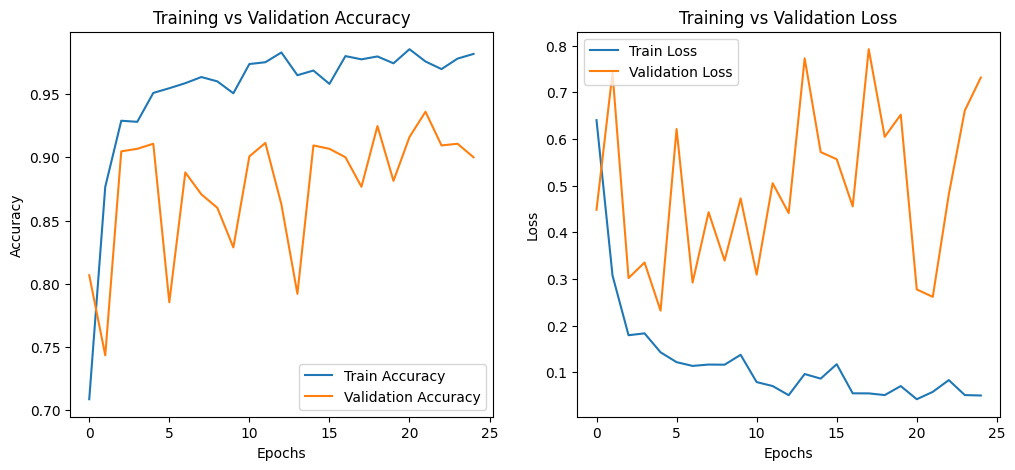
\includegraphics[width=\columnwidth]{AIML}
    \caption{Model training performance showing accuracy and loss over epochs}
    \label{fig:performance}
\end{figure}

\section{Conclusion}
In this study, we've taken a meaningful step toward simplifying plant identification by harnessing the power of deep learning. Our Convolutional Neural Network, trained on a rich dataset of 5,000 leaf images from five Indian plants—Tulsi, Money Plant, Lemon, Mango, and Rosa-senensis has shown how technology can shine a light on nature's diversity. By carefully designing the model and using tricks like data augmentation, we've built something that doesn't just work in theory but holds real promise for everyday use. It's exciting to think about how this could help farmers spot crops more easily, support conservation efforts, or even inspire students to explore the green world around them.
Looking back, this work isn't just about numbers or tech—it's about connecting with India's incredible plant life in a new way. We've created a tool that respects the uniqueness of each leaf while tackling a challenge that's been around for ages. Sure, there's room to grow, like adding more species or testing it in messier, real-world conditions, but what we've done here feels like a solid start. It's a blend of science and curiosity that could ripple out to fields like agriculture and education, making a small but real difference in how we understand and care for the plants that surround us.

\bibliographystyle{plain}
\bibliography{references}

\end{document} 